% chktex-file 13

\documentclass{article}
\usepackage{amsmath}
\usepackage{hyperref}
\usepackage{xcolor}
\usepackage{ulem}
\usepackage{graphicx}
\usepackage[margin=0.75in]{geometry}

\graphicspath{ {./images/} }

\definecolor{darkblue}{rgb}{0, 0, 20}

\hypersetup{
    colorlinks=true,
    urlcolor=darkblue,
    linkcolor=blue,
    filecolor=magenta,
    citecolor=blue,
}

\title{SelfPose3d: Self-Supervised Multi-Person Multi-View 3d Pose Estimation}
\author{Vinkle Srivastav, Keqi Chen, Nicolas Padoy}
\date{}
\setlength{\parindent}{0pt}

\begin{document}

\maketitle

\begin{center}\textbf{Accepted for CVPR 2024 (\href{https://arxiv.org/pdf/2404.02041}{Paper}) (\href{https://github.com/CAMMA-public/SelfPose3d}{GitHub})}\end{center}

This paper introduces a new self-supervised approach for estimating 3d poses of multiple people from multiple camera views. This method does not require 2d or 3d ground-truth poses for training and only uses generated 2d poses from a calibrated multi-view camera setup. The model first localizes all of the humans in the 3d space and their 3d root joint, a mid-hip point. Then, the 3d pose is generated for each 3d root joint.

\section*{Motivation}

Current state-of-the-art methods are either learning-based, which require 2d or 3d ground-truth poses from a dense camera system, or optimization-based, which don't rely on ground-truth but underperform in comparison. This method attempts to combine the strengths of both by training on 2D pose views from multiple cameras, which are easier to obtain than 3d ground-truth poses.

\begin{center}
    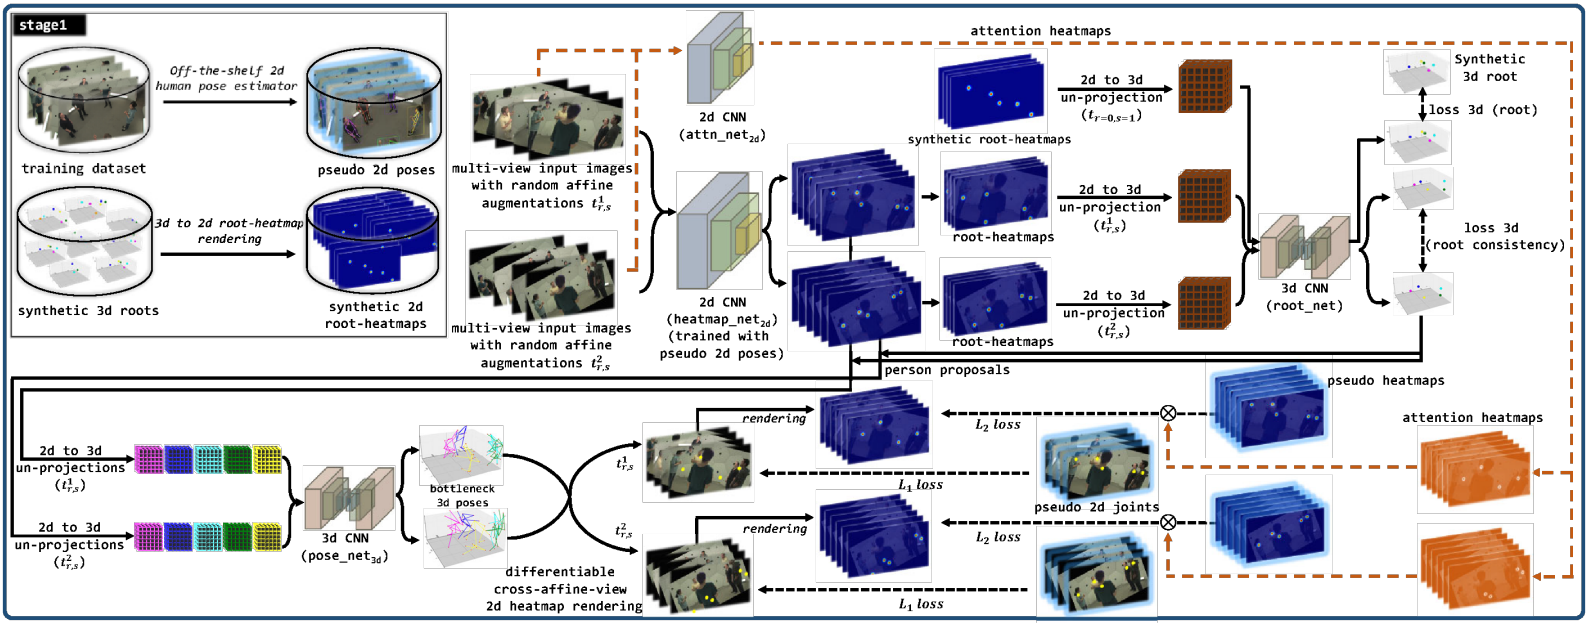
\includegraphics[scale=0.4]{selfpose3d-1.png}
\end{center}

\section*{Method}

\begin{enumerate}
    \item \textbf{3D Root Localization}
    
    A 2d root joint heatmap is generated from each view using a 2D CNN. Then, the 2D heatmaps are triangulated to build a 3d feature volume for the person proposals using a 3D CNN.

    \item \textbf{3D Pose Estimation}
    
    The 3d poses are predicted by passing the person proposals and 2d root heatmaps through a 3D CNN. During training, geometric constraints are enforced by projecting the 3d poses back into 2d space across affine-transformaed views.
    
    \item \textbf{Adaptive Supervision Attention}
    
    Attention is used to guide the training in occluded scenarios. For example, the 2d pose estimation may generate innacurate labels when occluded and the 3d-to-2d projection will output 2d joints, even when the person is occluded from that view. Their solution was soft attention for heatmap supervision and hard attention for joint loss.
\end{enumerate}

\begin{center}
    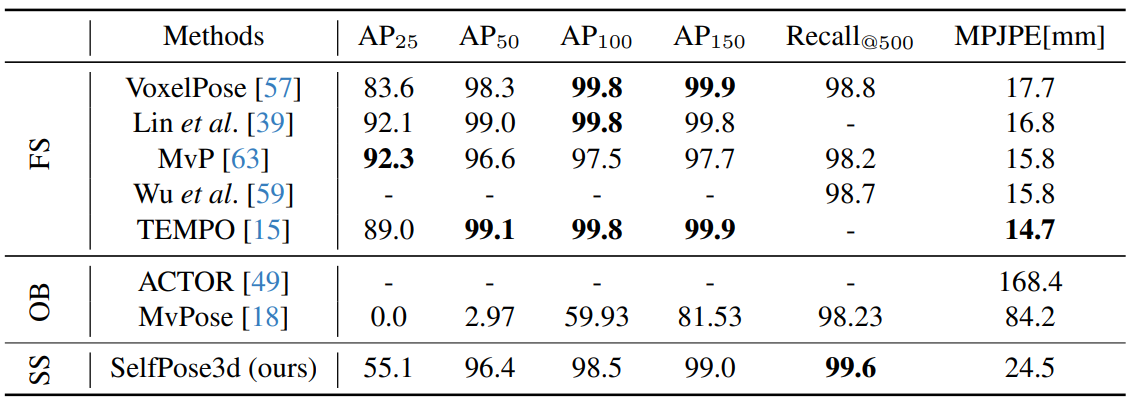
\includegraphics[scale=0.4]{selfpose3d-2.png}
\end{center}

\section*{Limitations}

\begin{enumerate}
    \item Occasionally hallucinates extra humans even in an isolated environment, as shown in the supplementary material compared to the fully-supervised VoxelPose
    \item The performance of the off-the-shelf 2d pose estimator constrains the model's accuracy, as the model builds the resulting 3d pose from the initial multi-view 2d pose
    \item May not handle heavily occluded environments where a person may not be visible to most of the cameras (trained on datasets that include multiple people and varying views but not occlusion-heavy environments)
\end{enumerate}

\begin{center}
    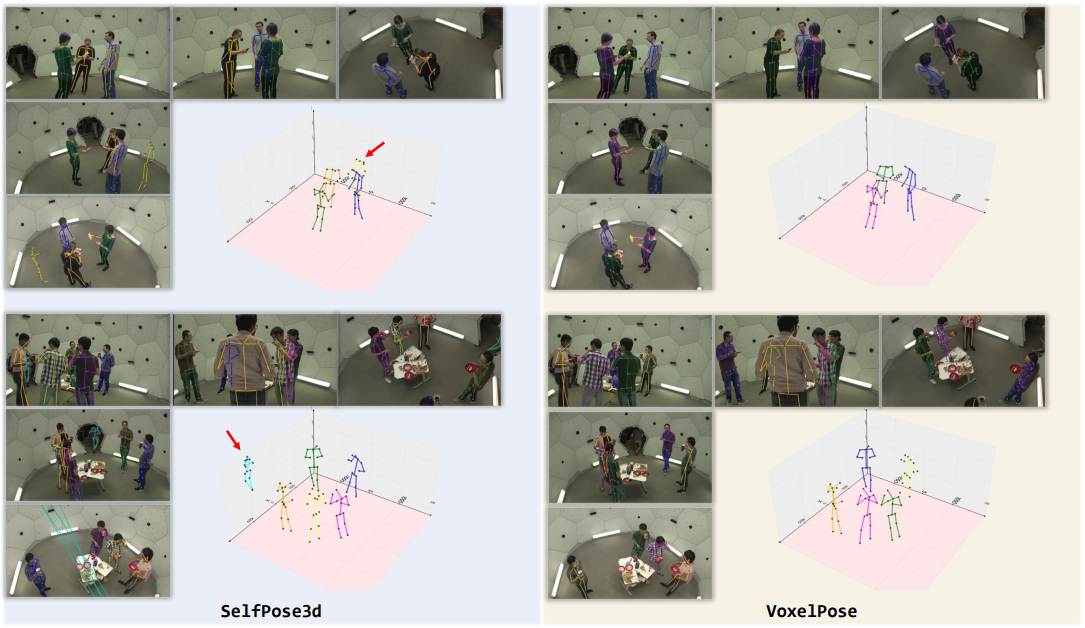
\includegraphics[scale=0.6]{selfpose3d-3.png}
\end{center}

\end{document}